Quando parliamo di equilibrio chimico omogeneo, con \textit{omogeneo} intendiamo che tutti i composti presenti nella reazione (reagenti e prodotti) sono nella stessa fase, con \textit{equilibrio} intendiamo che a un certo punto si raggiunge una situazione in cui apparentemente non varia più la reazione.
\subsection{La costante di equilibrio}
Consideriamo la reazione tra idrogeno gassoso e iodio gassoso (cosa non naturale per lo iodio in quanto è un solido. Ciò significa che lo abbiamo riscaldato per portarlo in fase vapore):

$$\ce{H_2(g) + I_2(g) <--> 2HI(g)}$$
\vspace{-1cm}\begin{figure}[htp]
    \centering
    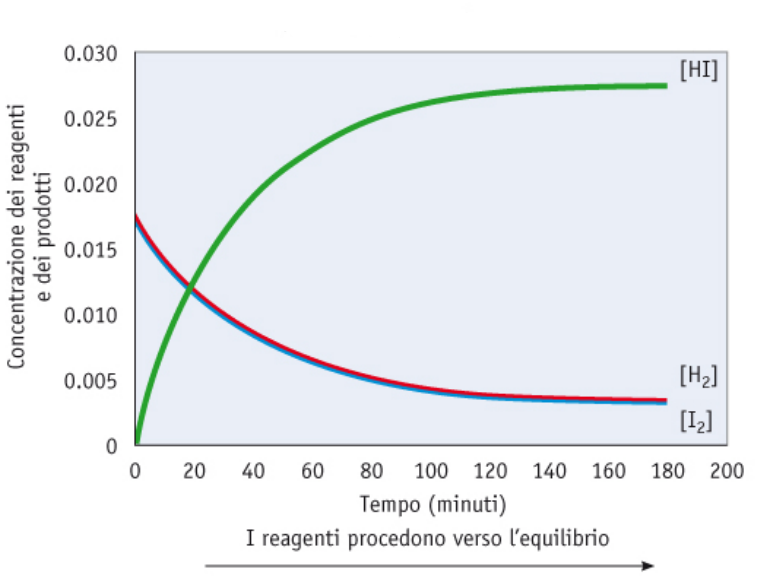
\includegraphics[width=10cm]{immagini/equilibrio_chimico.png}
\end{figure}

Il significato della doppia freccia è che la reazione può procedere in entrambi i sensi: sia da destra verso sinistra che da destra verso sinistra.

I due reagenti considerati danno luogo alla formazione di acido iodidrico, gassoso anch'esso.

L'equilibrio allora è omogeneo perché il prodotto ed entrambi i reagenti sono nella stessa fase.

Il grafico ci mostra che in questa particolare reazione le concentrazioni iniziali dei due reagenti sono uguali (non è necessario, ma conviene), mentre quella iniziale del prodotto è zero, cioè non c'è prodotto al tempo $t=0$.

Appena mescoliamo i reagenti e li facciamo reagire, immediatamente si forma acido iodidrico, ossia la reazione procede da sinistra verso destra.

Nell'istante in cui abbiamo già dell'acido iodidrico formato, piano piano parte la reazione opposta: l'acido si ridissocia per ridare nuovamente i reagenti.

Dato che ciò avviene subito, il processo sarà continuo.

Chiaramente alla fine ci sarà una parte dei reagenti che non ha reagito (o meglio, reagiscono ma poi si ridissociano). Le concentrazioni finali di H$_2$, I$_2$ e HI dipenderanno dalle concentrazioni iniziali di idrogeno e iodio.

\E importante che questa processo avvenga a temperatura fissata.

Si dimostra poi che il rapporto tra la concentrazione (indicata con le parentesi quadre) al quadrato del prodotto HI\footnote{eleviamo perché avevamo coefficiente stechiometrico pari a 2, cioè il coefficiente diventa esponente.} e il prodotto delle concentrazioni dei reagenti (ognuna elevata a 1 perché il loro coefficiente stechiometrico è 1) resta costante nel tempo, ossia è come se non cambiasse per le concentrazioni:

$$\rm \frac{[HI]^2}{[H_2] \cdot [I_2]}=\textit{cost}$$

In questa fase diciamo che il sistema ha raggiunto l'equilibrio, cioè quando la reazione è in equilibrio tale rapporto non cambia più.

Inoltre possiamo anche partire da concentrazioni diverse tra loro dei reagenti. Ciò che cambierà sarà l'HI finale, ma quel rapporto rimane invariato, a patto che sia mantenuta fissa la temperatura.

Il valore di tale rapporto si chiama \textbf{costante di equilibrio}.

La reazione di ri-dissociazione ha una sua velocità, che è inizialmente diversa dalla reazione di partenza. Da un punto di vista cinetico possiamo dire che abbiamo raggiunto l'equilibrio quando la velocità di trasformazione dei reagenti in prodotti e quella dei prodotti in reagenti si eguagliano. A quel punto si dice che il sistema ha raggiunto l'equilibrio chimico, cioè alla fine le velocità saranno uguali.

Chiaramente anche questo è un equilibrio dinamico, non statico. Ciò significa che le concentrazioni sono fissate, non cambiano, ma ciononostante dell'idrogeno e dello iodio continueranno a reagire per formare dell'acido iodidrico e dell'acido iodidrico si dissocerà per ripristinare idrogeno e iodio in modo continuo. Quindi le reazioni non si fermano, ma non ce ne accorgiamo perché le quantità non cambiano, ossia da un punto di vista delle concentrazioni diciamo che queste sono ormai costanti.

Inoltre in questa reazione non cambia il numero di moli: due moli di reagenti danno due moli di prodotto. Si tratta di un caso particolare, in generale il numero di moli tra reagenti e prodotti varierà.

\vspace{0.2cm}Consideriamo adesso questa reazione:

$$\ce{2NO(g) + 2H_2(g) <--> 2H_2O(g) + N_2(g)}$$

In essa a due moli di ossido di azoto aggiungiamo due moli di idrogeno, per un totale di 4 moli. Tuttavia otteniamo due moli di acqua più una di azoto, per un totale di 3 moli soltanto.

Partiamo quindi da 4 moli di reagenti e otteniamo 3 moli di prodotti, dunque questa è una reazione in cui il numero di moli cambia. \E però anche questa una reazione di equilibrio, pertanto diremo che essa è in equilibrio quando sia temperatura e pressione fissate all'inizio, che le concentrazioni, sono costanti.

Una volta raggiunto l'equilibrio non si otterrà ulteriore reagente. Se però rompiamo l'equilibrio sottraendo un prodotto, la reazione cercherà di ripristinare ciò che ha sottratto, ovvero la reazione ripartirà producendo il reagente sottratto.

\vspace{0.2cm}Da un punto di vista cinetico, affinché due o più molecole reagiscano è necessario che

\begin{itemize}
    \item Le molecole si urtino, quindi non possiamo lavorare con sistemi assolutamente ideali in cui i gas sono rarefatti e si comportano come se fossero l'unico presente, perché in tali condizioni non ci sarebbero urti;
    \item L'urto sia efficace, ossia deve dare luogo ad atto reattivo. Per avvenire ciò le molecole devono possedere energia sufficiente per produrre i prodotti (atto reattivo). Ovviamente solo una percentuale delle molecole possiederà tale energia.

    Si osserva che più il sistema è concentrato, maggiore è la probabilità che ci siano molecole che si urtino.
\end{itemize}

Inoltre la velocità della reazione è proporzionale alla concentrazione, quindi all'inizio è massima la velocità verso destra, perché abbiamo massima concentrazione. Nell'istante in cui la reazioni parte, diminuisce la concentrazione dei reagenti e inizia a crescere quella dei prodotti, dunque col procedere della reazione la velocità verso destra diminuisce e aumenta la velocità verso sinistra. Quando queste due velocità sono uguali siamo all'equilibrio.
\subsection{La legge delle masse}
Cerchiamo di capire da dove venga l'idea di un quoziente di reazione in cui al numeratore ci sono le concentrazioni dei prodotti e al denominatore quelle dei reagenti, elevate ciascuna per il proprio coefficiente stechiometrico.

Va da notare che stiamo lavorando con speci in fase gassosa, quindi ancora prima delle concentrazioni conosciamo le pressioni parziali di queste speci, date dal valore delle tensioni di vapore proprie delle sostanze pure per la frazione molare. Ragioniamo quindi in termini di pressione parziale esercitata da ciascuna specie gassosa.

Consideriamo due reagenti A e B, che reagiscono (in una reazione di equilibrio) per produrre i prodotti C e D:

$$\ce{\alpha A + \beta B <--> \gamma C + \delta D}$$

dove $\alpha$, $\beta$, $\gamma$ e $\delta$ sono i coefficienti stechiometrici. A, B, C e D sono speci chimiche gassose del sistema in equilibrio.

Indichiamo poi con $G_A^0$, $G_B^0$, $G_C^0$ e $G_D^0$ le energie libere molari standard\footnote{L'energia libera di Gibbs (o entalpia libera) è una funzione di stato usata per rappresentare l'energia libera, cioè il lavoro che il sistema può compiere sull'ambiente. \E definita come $G(T,P,n)=H-TS$.} (cioè a 25° C e e 1 atm) delle relative speci.

Indicheremo con $G_A$, $G_B$, $G_C$ e $G_D$ le energie libere molari a 25° C ma rispetto alle pressioni parziali finali di quando abbiamo raggiunto l'equilibrio.

Immaginiamo di avere eseguito una reazione e di essere passati da uno stato 1 a uno stato 2, in cui lo stato iniziale è a condizioni standard e lo stato finale è a condizioni di equilibrio, quindi ogni specie inizialmente aveva la pressione di 1 atm e alla fine avrà la pressione parziale $P_A$, $P_B$, $P_C$ o $P_D$. La variazione di energia libera in questa reazione sarà data da

$$\Delta G = RT \ln \frac{P_2}{P_1}, \quad \Delta G = G - G^0$$

La variazione di energia libera per ogni specie sarà

$$\Delta G_A = \alpha G_A - \alpha G_A^0 = \alpha RT \ln \frac{P_A}{1}$$

Segue che

$$ \alpha G_A = \alpha G_A^0  + \alpha RT \ln P_A$$

Analogamente
$$\beta G_B = \beta G_B^0  + \beta RT \ln P_B,
\quad
\gamma G_C = \gamma G_C^0  + \gamma RT \ln P_C,
\quad
\delta G_D = \delta G_D^0  + \delta RT \ln P_D$$

Possiamo allora calcolare un $\Delta G$ della reazione, dato dalla variazione di energia libera dei prodotti meno la variazione di energia libera dei reagenti.
$$\Delta G_{reazione} = (\gamma G_C + \delta G_D) - (\alpha G_A + \beta G_B)$$

sostituendo
$$\Delta G = (\gamma G_C^0  + \gamma RT \ln P_C + \delta G_D^0  + \delta RT \ln P_D) - 
(\alpha G_A^0  + \alpha RT \ln P_A + \beta G_B^0  + \beta RT \ln P_B)$$

$$\implies \Delta G = \gamma G_C^0 + \delta G_D^0 - \alpha G_A^0 - \beta G_B^0 + RT \ln \frac{P_C^{\gamma} \cdot P_D^{\delta}}{P_A^{\alpha} \cdot P_B^{\beta}}$$

Va da notare che l'argomento del logaritmo è il prodotto delle pressioni dei prodotti, diviso il prodotto delle pressioni parziali dei reagenti, dove ciascuna di queste pressioni è elevata per il proprio coefficiente stechiometrico.

Quando la reazione raggiunge l'equilibrio la variazione di energia libera è pari a zero: $\Delta G = 0$. Inoltre Poniamo
$$\Delta G^0 = \gamma G_C^0 + \delta G_D^0 - \alpha G_A^0 - \beta G_B^0 $$

Segue che

$$\Delta G^0 = -RT \ln \frac{P_C^{\gamma} \cdot P_D^{\delta}}{P_A^{\alpha} \cdot P_B^{\beta}}$$

A $T$ costante $\Delta G^0$ è un numero. Ne segue che anche l'argomento del logaritmo sarà uguale a una costante, la quale è funzione delle pressioni parziali. Tale costante è detta \textit{costante di reazione} $k_p$. L'espressione allora diventa

$$\frac{P_C^{\gamma} \cdot P_D^{\delta}}{P_A^{\alpha} \cdot P_B^{\beta}} = k_p
\quad\big(\text{da cui }
\Delta G^0 = -RT\ln k_p\big)\footnotemark$$

\footnotetext{Questa implicazione verrà usata in un secondo momento, quando ricaveremo l'equazione di Nernst in elettrochimica.}

Se la costante $k_p$ viene espressa in funzione delle concentrazioni diventa il rapporto delle concentrazioni visto all'inizio e che non cambia nonostante le concentrazioni iniziali. Tale risultato rappresenta la legge delle masse\footnote{Nei testi viene riportata come "Legge di azione di massa".}, la quale afferma che

\vspace{0.2cm}"\textit{In una reazione che ha raggiunto l'equilibrio, il rapporto tra il prodotto delle concentrazioni dei prodotti e quello dei reagenti, ciascuna elevata al proprio coefficiente stechiometrico, è una costante.}"

\vspace{0.2cm}Quindi, qualunque siano le condizioni iniziali, purché sia fissata la temperatura, il valore della costante $k_p$ non cambia per ogni reazione, cioè ogni reazione ha la sua costante che varia se cambia la temperatura, ma che non varia anche se cambiano le concentrazioni di reagenti e di prodotti.

Va da notare che le pressioni parziali che figurano in essa sono quelle all'equilibrio e non quelle iniziali. Analogamente se la esprimiamo con le concentrazioni.
\subsection{Relazione tra $\boldsymbol{k_p}$ e $\boldsymbol{k_c}$}
Stiamo parlando di equilibri in fase gassosa e quindi di reazioni in fase gassosa, nonché di pressioni parziali di ciascuno dei componenti. Noi però siamo abituati a lavorare in soluzione, pertanto laddove fosse possibile vogliamo capire come fare per ragionare su equilibri in soluzione acquosa (per possibile si intende avere speci che si sciolgono in acqua). Quello che vogliamo quindi capire è se c'è una relazione tra la costante di equilibrio in funzione delle pressioni parziali $k_p$ e la costante di equilibrio in funzione della concentrazione $k_c$.

La $k_p$ della reazione è
$$k_p = \frac{P_C^{\gamma} \cdot P_D^{\delta}}{P_A^{\alpha} \cdot P_B^{\beta}}$$

Dall'equazione di stato dei gas si ha

$$PV=nRT \implies P=\frac{n}{V}RT \implies P=c \cdot RT$$

Se indichiamo con [A], [B], [C] e [D] le varie concentrazioni, la $k_p$ sarà

$$k_p = \frac{[\text{C}]^{\gamma} [\text{D}]^{\delta}}{[\text{A}]^{\alpha} [\text{B}]^{\beta}} \cdot \frac{(RT)^{\gamma} (RT)^{\delta}}{(RT)^{\alpha} (RT)^{\beta}}$$

Poniamo

$$k_c = \frac{[\text{C}]^{\gamma} [\text{D}]^{\delta}}{[\text{A}]^{\alpha} [\text{B}]^{\beta}}
\quad;\quad
\Delta n= (\gamma + \delta - \alpha - \beta)$$

Scriveremo che
$$k_p = k_c \cdot (RT)^{\Delta n}$$

$\Delta n$ è la variazione del numero di moli. Se le moli di reagenti sono uguali in numero a quelle dei prodotti $\Delta n$ sarà pari a zero, per cui $k_p = k_c$. In caso contrario, cioè se cè variazione del numero di moli, $\Delta n \neq 0$ e $k_p \neq k_c$.

\vspace{0.2cm}\textbf{ES.1}
$$\ce{H_2 + I_2 <--> 2HI}, \quad \Delta n = 0 \implies k_p = k_c$$

\textbf{ES.2}
$$\ce{PCl_5  <--> PCl_3 + Cl_2}, \quad \Delta n = 1 \implies k_p = k_c - RT$$
